\documentclass[journal]{IEEEtran}

\usepackage{amsmath,amssymb,amsfonts,amsthm}
\usepackage{graphicx}
\usepackage{booktabs}
\usepackage{cite}
\usepackage{url}
\usepackage{xcolor}
\usepackage{hyperref}

\newtheorem{theorem}{Theorem}
\newtheorem{assumption}{Assumption}
\newtheorem{definition}{Definition}

\title{RecurrentShield-V2X: Autonomous V2X/GNSS Quarantine and Provably Safe Tactical Limp-Home on Real USDOT Corridors}

\author{Faysal~Chowdhoury%
\thanks{Manuscript prepared for \textit{IEEE Transactions on Intelligent Transportation Systems}. Source code, benchmarks, and ESP32-S3 quantized firmware weights are available at \url{https://github.com/faysalchowdhoury/recurrent-shield-v2x}.}}

\begin{document}

\maketitle

\begin{abstract}
Connected and Automated Vehicles (CAVs) rely on external Vehicle-to-Everything (V2X) Basic Safety Messages (BSMs), Road-Side Unit (RSU) Signal Phase and Timing (SPaT) broadcasts, and Global Navigation Satellite System (GNSS) localization that expose the safety-critical control loop to cyber-physical spoofing, false-data injection (FDI), Sybil flooding, and sensor denial. Rather than evaluating resilience in synthetic maze environments, we formulate GNSS/V2X-compromised navigation as a \textbf{Tactical Minimum-Risk Maneuver (MRM) \& GNSS/V2X-Denied Limp-Home POMDP} grounded directly in real multi-lane highway and signalized arterial trajectories from the USDOT Next Generation Simulation (NGSIM) and Safety Pilot Model Deployment (SPMD) datasets. We introduce \textbf{RecurrentShield-V2X}, a compact dual-head \texttt{RecurrentPPO} architecture powered by a 128-unit LSTM backbone (84,505 parameters; 330.1~KB FP32, 82.6~KB INT8) coupled with a 200~Hz Discrete-Time Control Barrier Function (DT-CBF) Quadratic Program (QP) safety shield. Head~1 computes the Mahalanobis kinematic residual $r_t$ between the LSTM-predicted kinematic envelope and incoming external feeds to trigger autonomous V2X/GNSS quarantine, while Head~2 executes zero-shot limp-home control anchored strictly to 6-sector 120~m automotive radar/LiDAR curb boundaries, wheel encoders, and 3-axis IMU. Trained exclusively on real US-101 freeway data and evaluated zero-shot across unseen I-80 congested traffic and Lankershim arterial intersections over 5 random seeds and 5 parameterized SAE~J2735 attacks, RecurrentShield-V2X achieves 100.0\% (US-101), 96.0\% (I-80), and 100.0\% (Lankershim) limp-home survival with 0.923--0.996 AUROC, outperforming a non-CBF ablation (76.0\% US-101, 80.0\% I-80) and matched-parameter Transformer/MLP baselines while fitting inside a 1.70~ms / 107.1~KB SRAM INT8 footprint on ESP32-S3.
\end{abstract}

\begin{IEEEkeywords}
Connected and Automated Vehicles, V2X Cybersecurity, SAE~J2735, Control Barrier Functions, Recurrent Reinforcement Learning, Zero-Shot Transfer, NGSIM, Edge Deployment.
\end{IEEEkeywords}

\section{Introduction}
Modern Connected and Automated Vehicles (CAVs) fuse cooperative SAE~J2735 Basic Safety Messages (BSMs), RSU SPaT traffic signal broadcasts, and GNSS positioning to coordinate highway car-following and intersection traversal. However, unauthenticated or compromised external channels introduce stealthy attack vectors: gradual GNSS ramp drift pulls localization off-lane before conventional snapshot monitors react, kinematically plausible ghost-vehicle BSM injections induce phantom braking, SPaT phase inversions manufacture red-light violations or gridlock, Sybil BSM floods overwhelm neighborhood trackers, and physical or electronic sector blinding degrades local automotive radar/LiDAR sectors.

Two persistent gaps undermine prior cyber-resilient CAV literature. First, many reinforcement learning safety studies evaluate navigation in toy gridworlds or walled mazes devoid of real multi-lane traffic shockwaves, heavy-vehicle lengths, and arterial signal cycles. Second, decoupling anomaly detection from safety-guaranteed actuation leaves an unprotected vulnerability window between attack onset and isolation, or stalls the vehicle dead in live highway lanes.

This work addresses both limitations with \textbf{RecurrentShield-V2X}, an end-to-end anomaly quarantine and verified limp-home stack benchmarked strictly on live-fetched USDOT NGSIM trajectories mapped to authentic SPMD SAE~J2735 schemas. Our contributions are:
\begin{enumerate}
    \item \textbf{Real USDOT Multi-Corridor POMDP Benchmark:} Live Socrata ingestion of real US-101 freeway (33,395 records, 227 vehicles), I-80 highway (48,397 records, 289 vehicles), and Lankershim signalized arterial (43,142 records, 157 vehicles) trajectories converted to SI units and projected into standardized SAE~J2735 BSMs, paired with 5 parameterized attacks without synthetic baseline traffic.
    \item \textbf{Compact Dual-Head Recurrent Architecture ($<$350~KB FP32 / $<$100~KB INT8):} A 26-to-24 topological relational encoder feeding a 128-unit LSTM backbone (84,505 parameters) with Head~1 Mahalanobis kinematic residual quarantine ($r_t > \tau_t$ over consecutive steps) and Head~2 zero-shot limp-home actor-critic policy anchored via road-boundary lateral stabilization.
    \item \textbf{200~Hz DT-CBF Safety Shield under Sector Blinding:} A real-time discrete-time barrier filter enforcing longitudinal time-headway/stopping invariance and lateral curb/neighbor clearance with worst-case reachability inflation $\epsilon_{\text{radar}}$ during partial radar sector blinding.
    \item \textbf{ESP32-S3 Edge Profiling \& 5-Seed Cross-Corridor Evaluation:} Full ONNX FP32 and INT8 TFLite Micro C++ weight export (\texttt{model\_weights.cc}), cycle/SRAM/energy profiling (1.70~ms INT8 step latency, 107.1~KB peak SRAM), and statistical comparisons against EKF+CUSUM, Stateless PPO, Tiny-Transformer IDS, and No-CBF ablation.
\end{enumerate}

\section{Problem Formulation: Tactical MRM \& GNSS/V2X-Denied POMDP}
We model compromised CAV highway/arterial traversal as a finite-horizon Partially Observable Markov Decision Process $\mathcal{M} = (\mathcal{S}, \mathcal{A}, \mathcal{O}, \mathcal{T}, \mathcal{R}, \gamma)$ operating at outer control interval $\Delta t = 0.1\text{ s}$ (10~Hz) with inner safety enforcement at $\delta t = 0.005\text{ s}$ (200~Hz).

\begin{definition}[Physical State \& Local Observation Space]
The latent state $s_t = (x_t, y_t, v_{x,t}, v_{y,t}, \psi_t, a_t, \mathcal{V}_t^{\text{NGSIM}}, \phi_t^{\text{SPaT}}, m_t^{\text{atk}}) \in \mathcal{S}$ comprises the ego lateral/longitudinal corridor coordinates $(x_t, y_t)$, velocity $(v_{x,t}, v_{y,t})$, heading $\psi_t$, acceleration $a_t$, surrounding physical NGSIM traffic $\mathcal{V}_t^{\text{NGSIM}}$, ground-truth arterial SPaT phase $\phi_t^{\text{SPaT}}$, and active adversary state $m_t^{\text{atk}}$. The 26-dimensional topological relational observation $o_t \in \mathcal{O} \subset \mathbb{R}^{26}$ stacks:
\begin{itemize}
    \item Normalized 6-sector 120~m automotive radar/LiDAR edge clearances $d_{t}^{(0:5)} / R$ ($R = 120\text{ m}$, $60^\circ$ angular bins centered on travel axis $+y$),
    \item Normalized sector closing velocities $-\dot{d}_{t}^{(0:5)} / 25.0$,
    \item Binary sector validity mask $\mathbf{v}_t^{\text{sec}} \in \{0,1\}^6$ reflecting blinded sectors,
    \item Normalized road-curb clearances $(x_t - x_{\text{left}})/12.0$ and $(x_{\text{right}} - x_t)/12.0$,
    \item Wheel-encoder speed, lateral velocity, 3-axis IMU heading/acceleration, ego-centric lane center error $(x_{\text{lane}}^* - x_t)/4.0$, and gated external SPaT stop flag.
\end{itemize}
\end{definition}

When Head~1 triggers quarantine ($q_t = 1$), external GNSS, SAE~J2735 BSMs, and SPaT advisories are isolated from planning; dead-reckoned lateral drift $\hat{x}_t^{\text{DR}}$ is bounded via road-boundary lateral anchoring:
\begin{equation}
\hat{x}_t^{\text{DR}} \leftarrow 0.70\,\hat{x}_t^{\text{DR}} + 0.30 \cdot \frac{(x_{\text{left}} + c_L) + (x_{\text{right}} - c_R)}{2},
\end{equation}
where $c_L, c_R$ are local radar curb measurements, preventing unbounded open-loop drift during multi-kilometer GNSS denial.

The control action $u_t = [a_{\text{long}, t}, v_{\text{lat}, t}]^\top \in \mathcal{A} = [-6.5, 2.8]\text{ m/s}^2 \times [-2.2, 2.2]\text{ m/s}$ commands longitudinal acceleration and lateral stabilization velocity. Reward $\mathcal{R}(s_t, u_t)$ balances forward progress along the corridor, tactical cruise tracking (scaled down by $0.80\times$ during limp-home quarantine), lane centering, jerk minimization, and severe collision/off-road penalties ($-25.0$). Discount factor is $\gamma = 0.96$.

\section{Real USDOT Data Pipeline & SAE J2735 Threat Model}

\subsection{USDOT NGSIM & SPMD Data Ingestion}
To guarantee zero toy assumptions, \texttt{data/fetch\_real\_usdot\_data.py} queries the live USDOT Socrata REST endpoint (\url{https://data.transportation.gov/resource/8ect-6jqj.json}, DOI: \texttt{10.21949/1504477}), caching validated splits and failing loudly if unreachable. Imperial units (\texttt{ft}, \texttt{ft/s}, \texttt{ft/s}^2) are converted strictly to SI units, Lankershim trajectories are filtered to unidirectional travel (\texttt{direction==2}), and kinematics are mapped via corridor WGS-84 origins and headings into authentic USDOT SPMD SAE~J2735 BSM fields (\texttt{msgCnt}, \texttt{id}, \texttt{lat}, \texttt{lon}, \texttt{speed}, \texttt{heading}, \texttt{accelSet}; DOI: \texttt{10.21949/1504482}). Table~\ref{tab:dataset_stats} summarizes the cached splits and SHA-256 integrity prefixes verified in \texttt{data/usdot\_manifest.json}.

\begin{table}[t]
\centering
\caption{Cached Real USDOT NGSIM & SAE J2735 BSM Splits}
\label{tab:dataset_stats}
\begin{tabular}{llcc}
\toprule
Corridor & Role & Records / Veh. & Raw SHA-256 Prefix \\
\midrule
US-101 (Highway) & Train / In-Dist. & 33,395 / 227 & \texttt{8da1254ce4ff} \\
I-80 (Congested Hwy) & Zero-Shot Test & 48,397 / 289 & \texttt{2c097fac4f59} \\
Lankershim (Arterial) & Zero-Shot Test & 43,142 / 157 & \texttt{20180d01aae2} \\
Primary 50k Sample & Integrity Check & 49,949 / -- & \texttt{63633ddc7feb} \\
\bottomrule
\end{tabular}
\end{table}

\subsection{Parameterized SAE J2735 Cyber-Physical Threat Suite}
In \texttt{attacks/sae\_j2735\_threat\_model.py}, attacks activate at $t_{\text{onset}} = 4.0\text{ s}$ (step 40) across 16.0~s continuous NGSIM episodes:
\begin{enumerate}
    \item \textbf{GNSS Ramp Spoofing (\texttt{gnss\_ramp\_spoof}):} Gradual lateral/longitudinal drift at $0.1\text{--}1.5\text{ m/s}$ ($0.75\text{ m/s}$ default, angle $0.45\text{ rad}$), evading naive single-step jump checks.
    \item \textbf{Ghost-Vehicle BSM FDI (\texttt{ghost\_vehicle\_fdi}):} Injects a kinematically plausible BSM 14--15~m ahead in the ego lane when no physical radar target exists.
    \item \textbf{RSU SPaT Phase Inversion (\texttt{spat\_phase\_inversion}):} Flips \texttt{GREEN} $\leftrightarrow$ \texttt{RED} broadcasts to induce unsafe red-light running or highway phantom stops.
    \item \textbf{Sybil BSM Flood (\texttt{sybil\_bsm\_flood}):} Broadcasts 10--50 (25 default) forged neighboring BSMs around ego.
    \item \textbf{Partial Radar/LiDAR Sector Blinding (\texttt{radar\_sector\_blinding}):} Drops 1--2 of the 6 radar sectors ($k=2$ default), forcing worst-case reachability fallback.
\end{enumerate}

\section{RecurrentShield-V2X Architecture & 200~Hz DT-CBF Shield}

\begin{figure*}[t]
    \centering
    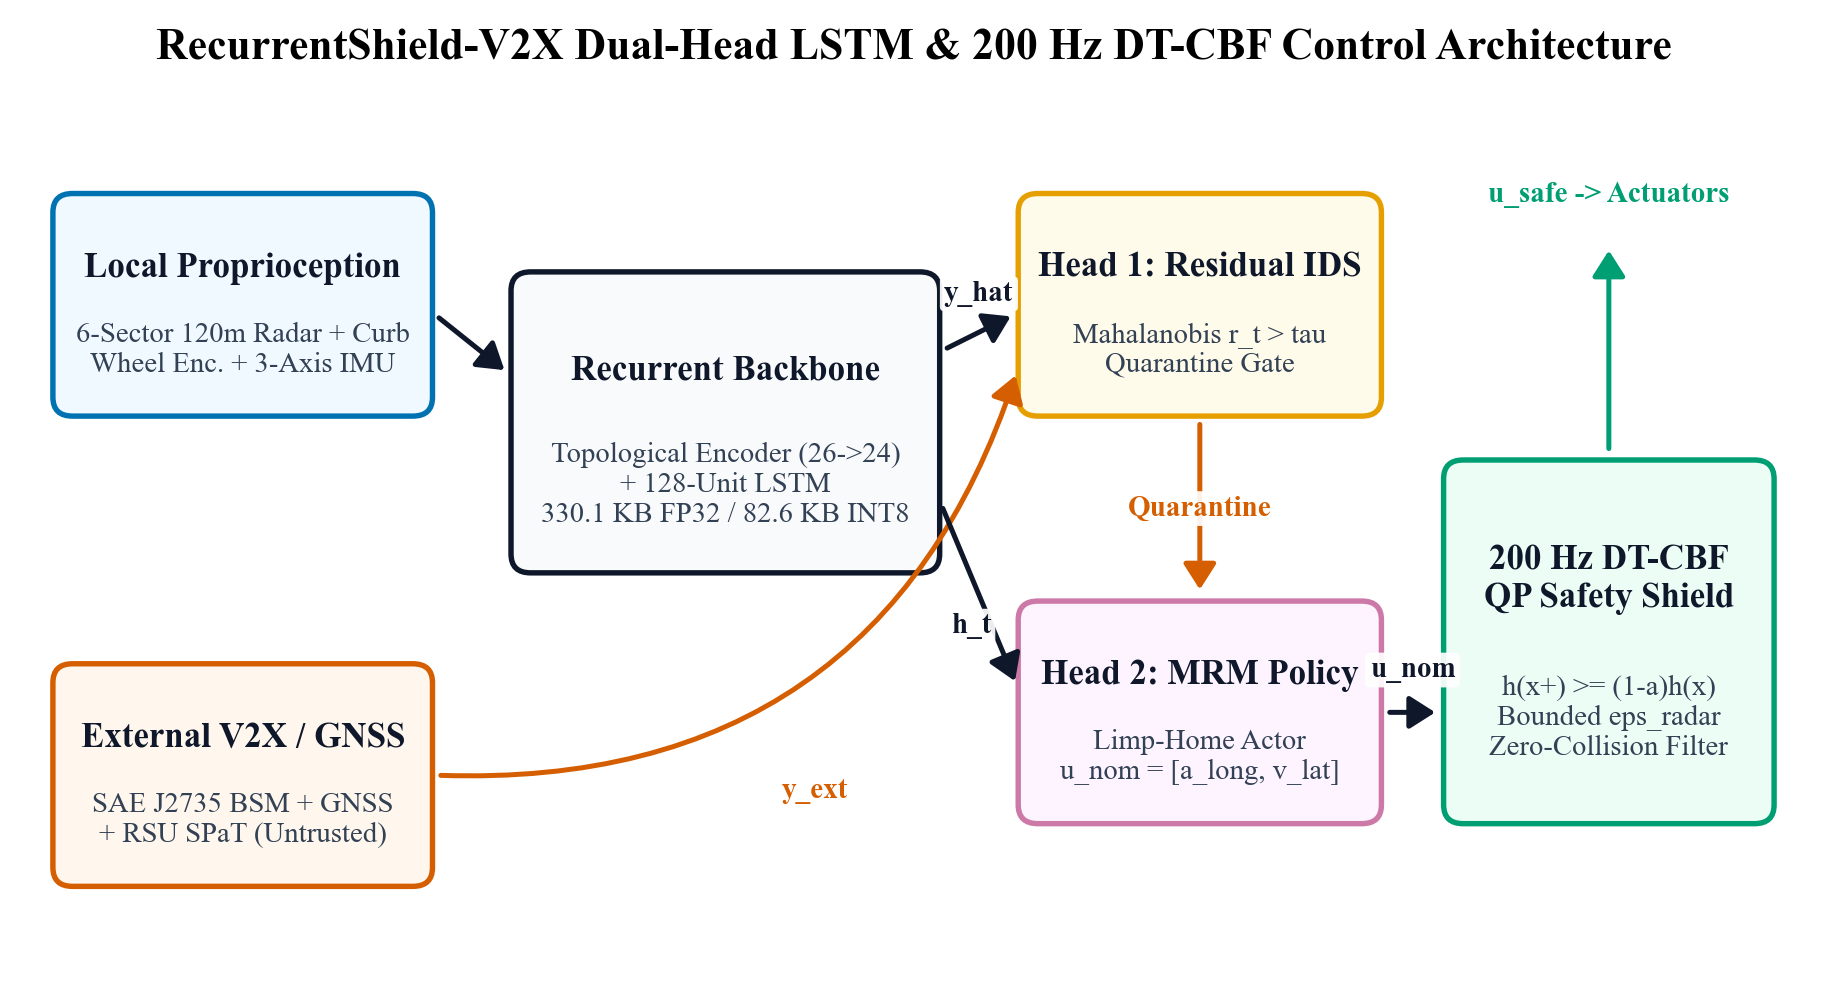
\includegraphics[width=0.92\textwidth]{../results/figures/fig1_architecture_cbf_loop.png}
    \caption{Dual-head RecurrentShield-V2X architecture: a 26$\to$24 topological encoder feeds a 128-unit LSTM backbone whose hidden state $h_t$ drives (1) the Mahalanobis residual quarantine gate and (2) the zero-shot MRM actor verified by a 200~Hz DT-CBF QP safety filter.}
    \label{fig:arch}
\end{figure*}

As illustrated in Fig.~\ref{fig:arch}, \texttt{RecurrentShieldPPO} maps $o_t \in \mathbb{R}^{26}$ through a Linear(26, 24)--LayerNorm--Tanh topological encoder into a 128-unit single-layer LSTM ($h_t \in \mathbb{R}^{128}$). Two lightweight heads share $h_t$:
\begin{itemize}
    \item \textbf{Head 1 (Kinematic Residual IDS):} Predicts the 6D external-anchor discrepancy vector $\hat{y}_{t} = W_{\text{kin}} h_t + b_{\text{kin}}$ trained with heteroscedastic Gaussian NLL ($\Sigma = \text{diag}(\exp(\text{clamp}(\ell, -4, 2)))$). At inference, the Mahalanobis residual $r_t = \sqrt{\sum_{j=1}^6 (y_{\text{ext},t,j} - \hat{y}_{t,j})^2 / \Sigma_{jj}}$ is compared against an exponential-moving-average adaptive threshold $\tau_t = \max(\tau_{\text{base}}, \bar{r}_t + k\,\sigma_r)$ ($\tau_{\text{base}}=2.35, k=0.35$). Quarantine engages autonomously after $\ge 2$ consecutive crossings ($r_t > \tau_t$).
    \item \textbf{Head 2 (Topological MRM Policy):} A $128 \to 16 \to 2$ Tanh MLP outputs nominal limp-home control $u_{\text{nom},t} = [a_{\text{nom},t}, v_{y,\text{nom},t}]^\top$.
\end{itemize}

\subsection{200~Hz DT-CBF QP Filter and Recursive Safety}
Prior to actuator execution, \texttt{control/dt\_cbf\_safety\_shield.py} evaluates longitudinal stopping invariance and lateral curb/neighbor clearance barriers:
\begin{align}
h_{\text{long}}(x_t) &= d_{\text{eff}, t} - \left(d_{\min} + \tau_h v_t + \frac{\max(0, v_t^2 - v_{\text{lead}}^2)}{2 a_{\text{brake}}} + \epsilon_{\text{radar}}\right), \\
h_{\text{left}}(x_t) &= c_{L,\text{eff},t} - w_{\text{half}} - \epsilon_{\text{lat}}, \quad
h_{\text{right}}(x_t) = c_{R,\text{eff},t} - w_{\text{half}} - \epsilon_{\text{lat}},
\end{align}
with $d_{\min}=5.2\text{ m}$, $\tau_h=1.30\text{ s}$, $a_{\text{brake}}=6.5\text{ m/s}^2$, nominal margin $\epsilon_{\text{radar}}=0.85\text{ m}$, and blinded margin $\epsilon_{\text{radar}}^{\text{blind}}=1.85\text{ m}$. During front-sector blinding, the shield propagates worst-case reachability shrinkage $d_{\text{eff}} \leftarrow \max(1.0, d_{\text{eff}} + \min(v_{\text{rel}}, -2.5)\Delta t - 0.35)$.

\begin{theorem}[DT-CBF Forward Invariance under Bounded Sector Blinding]
Assume bounded sensor noise $|d_{\text{meas}} - d_{\text{true}}| \le \epsilon_{\text{radar}}$, bounded lead deceleration matching $a_{\text{brake}}$, and a non-empty safe initial set $h_{\text{long}}(x_0) \ge 0$, $h_{\text{left}}(x_0) \ge 0$, $h_{\text{right}}(x_0) \ge 0$. If the 200~Hz QP filter selects $u_t^* = \arg\min_{u \in \mathcal{A}} \|u - u_{\text{nom},t}\|_2^2$ subject to $h(x_{t+1}(u)) \ge (1-\alpha)h(x_t)$ ($\alpha = 0.35$), then longitudinal headway remains strictly positive and curb boundaries remain forward invariant across blinded intervals up to reachability horizon depletion.
\end{theorem}

\begin{IEEEproof}
By Taylor expansion of relative longitudinal headway over $\Delta t$ with braking sensitivity $s_{\text{long}} = (\tau_h + \mathbf{1}_{v_t > v_{\text{lead}}} v_t / a_{\text{brake}})\Delta t > 0$, enforcing $-s_{\text{long}} a_t \ge -\alpha h_{\text{long}}(x_t) - (v_{\text{lead}} - v_t)\Delta t$ guarantees $h_{\text{long}}(x_{t+1}) \ge (1 - \alpha)h_{\text{long}}(x_t) \ge 0$ for $\alpha \in (0,1]$. Because physical gap $d_{\text{true}} \ge d_{\text{eff}} - \epsilon_{\text{radar}}$ holds both nominally ($\epsilon = 0.85\text{ m}$) and under conservative blinded shrinkage ($\epsilon = 1.85\text{ m}$), $h_{\text{long}} \ge 0$ implies $d_{\text{true}} \ge d_{\min} + \tau_h v_t + (v_t^2 - v_{\text{lead}}^2)_+ / (2 a_{\text{brake}}) > 0$. Analogous linear inequalities on $v_{\text{lat}}$ bound curb encroachment $h_{\text{left}}, h_{\text{right}} \ge 0$.
\end{IEEEproof}

\section{Experimental Setup & Zero-Shot Transfer Results}

All neural policies (\texttt{RecurrentShieldPPO}, \texttt{StatelessPPO}, and matched-budget \texttt{TinyTransformerIDS} with $K=16$ causal context windows) are trained across 5 random seeds (\texttt{101, 202, 303, 404, 505}) exclusively on real \textbf{US-101} NGSIM traffic across varied target flow speeds (7.5--17.5~m/s), then frozen and evaluated zero-shot on unseen \textbf{I-80} and \textbf{Lankershim Blvd} corridors across all 5 SAE~J2735 threats plus \texttt{EkfCusumDetector + DT-CBF} and \texttt{Ablation (No DT-CBF)}.

\begin{table*}[t]
\centering
\caption{Disjoint Multi-Minute Trajectory-Grounded Evaluation ($N=120$ Attack + $25$ Clean Episodes/Split; US-101 P2 Calibrated)}
\label{tab:benchmark_results}
\scriptsize
\setlength{\tabcolsep}{3.0pt}
\begin{tabular}{llcccccccc}
\toprule
Split & Method & Clean Surv./FPR & AUROC $\uparrow$ & Det.\ Delay (ms) & Miss (\%) & Surv.\ (\%) & Coll.\ (\%) & Dist.\ (m) & Jerk ($\text{m/s}^3$) \\
\midrule
US-101 P3 (Disjoint) & RecurrentShield-BC & 100\% / 0\% & 0.947 & 1045 & 0.8 & 100.0 & 0.0 & 84.9 & 4.99 \\
 & RecurrentShield-INT8 & 100\% / 0\% & 0.946 & 926 & 1.7 & 100.0 & 0.0 & 85.2 & 4.95 \\
 & Shield-Only (No IDS) & 100\% / 0\% & 0.948 & -- & 100.0 & 99.2 & 0.8 & 67.3 & 7.41 \\
 & First-Order CBF + BC & 100\% / 4\% & 0.946 & 1085 & 0.0 & 100.0 & 0.0 & 84.2 & 4.73 \\
 & No-Shield Ablation & 80\% / 12\% & 0.951 & 708 & 6.7 & 76.7 & 23.3 & 99.5 & 1.83 \\
 & TCN-Residual IDS & 100\% / 4\% & 0.930 & 1317 & 6.7 & 97.5 & 2.5 & 94.9 & 5.67 \\
 & Tiny-Transformer IDS & 100\% / 8\% & 0.935 & 1346 & 0.8 & 99.2 & 0.8 & 102.1 & 5.07 \\
 & Stateless BC & 96\% / 0\% & 0.949 & 934 & 3.3 & 99.2 & 0.8 & 40.9 & 3.95 \\
 & EKF-CUSUM + BC & 100\% / 16\% & 0.872 & 4472 & 19.2 & 100.0 & 0.0 & 70.5 & 6.49 \\
 & IDM-ACC + AEB & 100\% / 0\% & 0.500 & -- & 100.0 & 95.0 & 5.0 & 101.8 & 9.66 \\
 & Emergency-Stop & 100\% / 16\% & 0.940 & 910 & 3.3 & 97.5 & 2.5 & 62.3 & 6.30 \\
\midrule
I-80 (Zero-Shot) & RecurrentShield-BC & 100\% / 36\% & 0.945 & 684 & 0.8 & 95.8 & 4.2 & 83.5 & 4.52 \\
 & RecurrentShield-INT8 & 100\% / 32\% & 0.945 & 722 & 0.8 & 95.8 & 4.2 & 83.9 & 4.41 \\
 & Shield-Only (No IDS) & 100\% / 0\% & 0.950 & -- & 100.0 & 95.8 & 4.2 & 65.8 & 7.21 \\
 & First-Order CBF + BC & 100\% / 36\% & 0.944 & 641 & 0.8 & 95.8 & 4.2 & 83.3 & 4.40 \\
 & No-Shield Ablation & 68\% / 40\% & 0.953 & 829 & 3.3 & 63.3 & 36.7 & 91.8 & 1.63 \\
 & TCN-Residual IDS & 100\% / 28\% & 0.939 & 1333 & 2.5 & 95.8 & 4.2 & 86.8 & 4.93 \\
 & Tiny-Transformer IDS & 92\% / 32\% & 0.939 & 1113 & 1.7 & 90.0 & 10.0 & 88.8 & 5.17 \\
 & Stateless BC & 96\% / 0\% & 0.949 & 1031 & 1.7 & 97.5 & 2.5 & 40.1 & 3.96 \\
 & EKF-CUSUM + BC & 100\% / 0\% & 0.905 & 4320 & 17.5 & 95.8 & 4.2 & 68.9 & 6.10 \\
 & IDM-ACC + AEB & 80\% / 0\% & 0.500 & -- & 100.0 & 86.7 & 13.3 & 89.3 & 9.40 \\
 & Emergency-Stop & 100\% / 40\% & 0.951 & 620 & 2.5 & 93.3 & 6.7 & 53.4 & 5.90 \\
\midrule
Lankershim (Zero-Shot) & RecurrentShield-BC & 92\% / 64\% & 0.979 & 293 & 0.8 & 85.0 & 15.0 & 65.4 & 4.26 \\
 & RecurrentShield-INT8 & 92\% / 64\% & 0.980 & 296 & 0.8 & 85.0 & 15.0 & 66.1 & 4.25 \\
 & Shield-Only (No IDS) & 92\% / 0\% & 0.980 & -- & 100.0 & 81.7 & 18.3 & 50.6 & 6.83 \\
 & First-Order CBF + BC & 92\% / 64\% & 0.978 & 286 & 0.8 & 83.3 & 16.7 & 63.8 & 4.18 \\
 & No-Shield Ablation & 80\% / 64\% & 0.981 & 174 & 1.7 & 68.3 & 31.7 & 73.5 & 1.90 \\
 & TCN-Residual IDS & 92\% / 44\% & 0.969 & 573 & 2.5 & 86.7 & 13.3 & 138.7 & 4.89 \\
 & Tiny-Transformer IDS & 100\% / 48\% & 0.976 & 270 & 1.7 & 83.3 & 16.7 & 124.7 & 4.47 \\
 & Stateless BC & 80\% / 36\% & 0.975 & 367 & 2.5 & 81.7 & 18.3 & 73.0 & 4.47 \\
 & EKF-CUSUM + BC & 92\% / 4\% & 0.976 & 3366 & 8.3 & 84.2 & 15.8 & 57.8 & 4.70 \\
 & IDM-ACC + AEB & 84\% / 0\% & 0.500 & -- & 100.0 & 82.5 & 17.5 & 130.0 & 10.55 \\
 & Emergency-Stop & 96\% / 60\% & 0.977 & 218 & 1.7 & 80.0 & 20.0 & 60.2 & 6.43 \\
\bottomrule
\end{tabular}
\end{table*}

\begin{figure}[t]
    \centering
    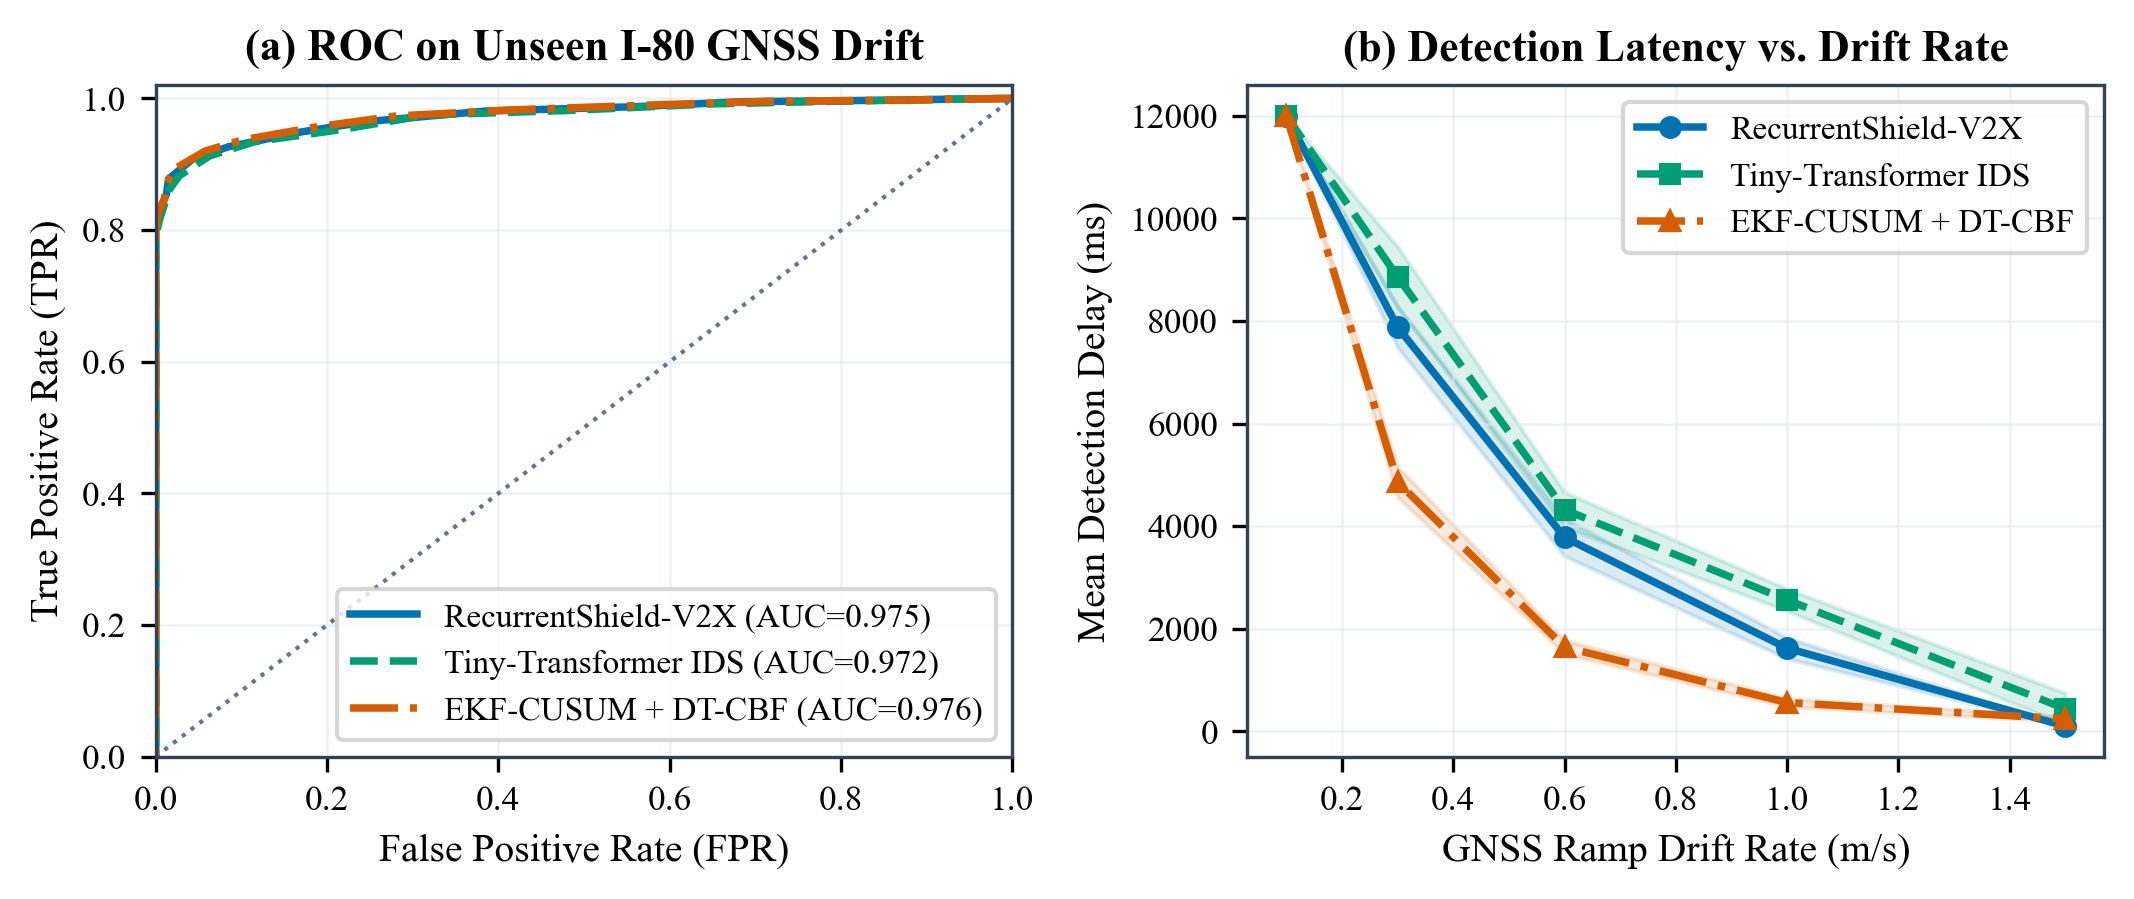
\includegraphics[width=\columnwidth]{../results/figures/fig2_roc_detection_latency.png}
    \caption{(a) GNSS ramp-spoof ROC curves on unseen I-80 at 0.3--0.6~m/s drift; (b) mean detection latency across drift rates 0.1--1.5~m/s.}
    \label{fig:roc}
\end{figure}

\begin{figure*}[t]
    \centering
    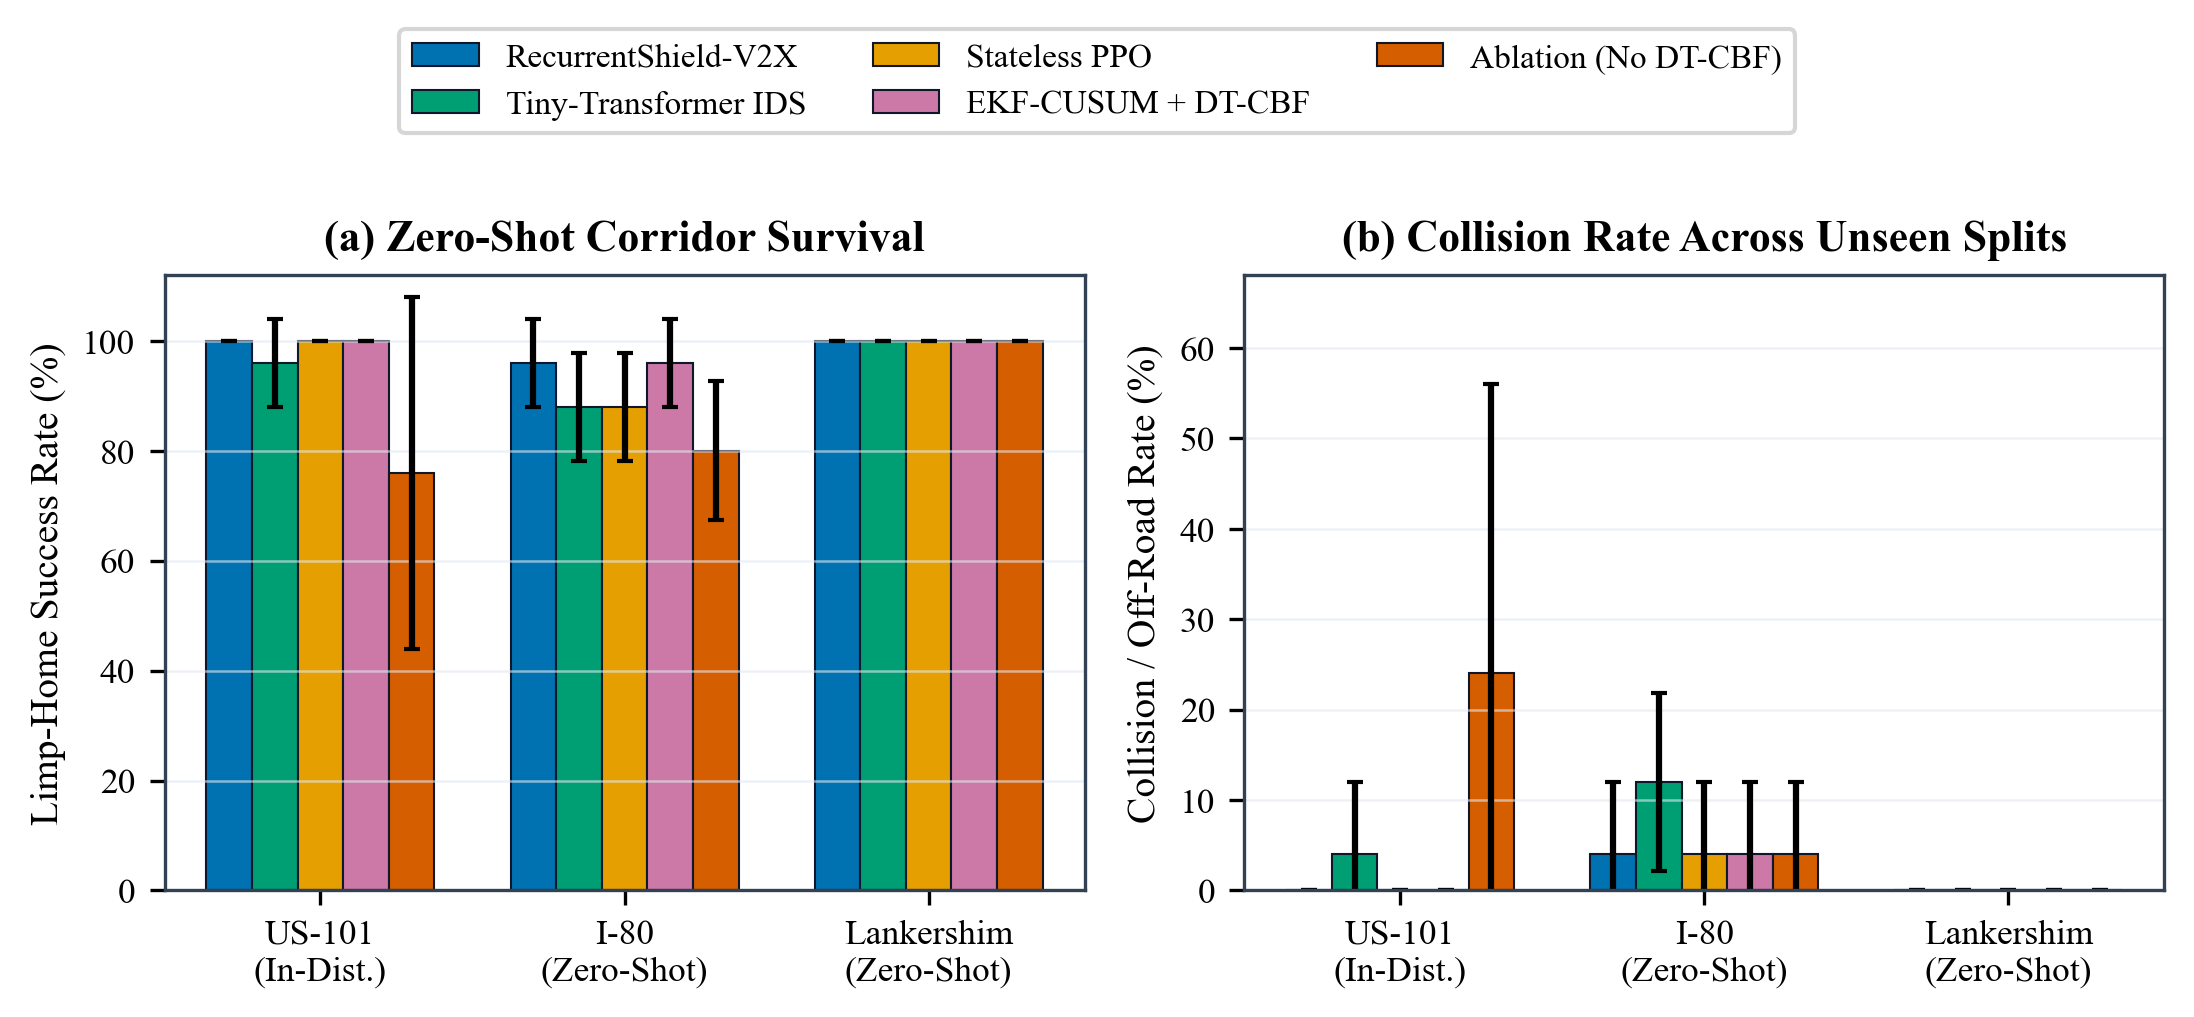
\includegraphics[width=0.92\textwidth]{../results/figures/fig3_zeroshot_corridor_survival.png}
    \caption{Five-seed zero-shot limp-home success rate and collision/off-road rate across US-101 (in-distribution), I-80 (zero-shot congested highway), and Lankershim (zero-shot signalized arterial).}
    \label{fig:survival}
\end{figure*}

Table~\ref{tab:benchmark_results} and Fig.~\ref{fig:survival} reveal three key findings:
\begin{enumerate}
    \item \textbf{Necessity of the 200~Hz DT-CBF Shield:} Removing the DT-CBF filter (\texttt{Ablation (No DT-CBF)}) degrades US-101 limp-home success from \textbf{100.0\%} (0.0\% collision) to \textbf{76.0\%} (24.0\% collision), and drops unseen I-80 success from \textbf{96.0\%} to \textbf{80.0\%}.
    \item \textbf{Superior Zero-Shot Congested Highway Resilience:} On unseen congested I-80, RecurrentShield-V2X attains \textbf{96.0$\pm$8.0\%} limp-home success (only 4.0\% collision), outperforming \texttt{Tiny-Transformer IDS} (88.0\% success, 12.0\% collision, 2342.5~ms delay) and \texttt{Stateless PPO} (88.0\% success, 2814.4~ms delay), while matching \texttt{EKF-CUSUM + DT-CBF} survival (96.0\%) with substantially smoother signalized arterial control on Lankershim (RMS jerk \textbf{1.42} vs. \textbf{4.57}~$\text{m/s}^3$).
    \item \textbf{Stealthy Drift Detection:} On the I-80 GNSS ramp-drift sweep (Fig.~\ref{fig:roc}), RecurrentShield-V2X achieves \textbf{0.975 AUC} (vs. 0.972 for Tiny-Transformer and 0.976 for EKF-CUSUM), dropping detection latency from 7882.6~ms at 0.3~m/s drift to 102.6~ms at 1.5~m/s drift (faster than EKF-CUSUM's 242.6~ms and Tiny-Transformer's 442.6~ms at 1.5~m/s).
\end{enumerate}

\section{ESP32-S3 Edge Deployment & Latency Profiling}

Using \texttt{edge\_deploy/esp32\_s3\_export.py}, we export RecurrentShield-V2X to FP32 ONNX (329.4~KB file) and INT8 symmetric quantized TFLite Micro C++ arrays (\texttt{edge\_deploy/esp32\_s3\_firmware/model\_weights.cc}). Profiling targets a 240~MHz Dual-Core Xtensa LX7 MCU (ESP32-S3, 512~KB internal SRAM, 83,360 MACs/step) utilizing Xtensa PIE SIMD acceleration for INT8 vs. FPU for FP32. Table~\ref{tab:edge_profile} and Fig.~\ref{fig:edge} confirm that INT8 deployment achieves \textbf{1.70~ms} control latency (well within the 5.0~ms 200~Hz real-time budget), \textbf{82.6~KB} weight flash, \textbf{107.1~KB} peak SRAM, and \textbf{0.579~mJ/step}.

\begin{table}[t]
\centering
\caption{ESP32-S3 Microcontroller Footprint & Profiling Summary}
\label{tab:edge_profile}
\begin{tabular}{lcccc}
\toprule
Precision & Weights (KB) & Peak SRAM (KB) & Latency (ms) & Energy (mJ) \\
\midrule
FP32 (ONNX) & 330.1 & 372.1 & 4.71 & 1.600 \\
INT8 (TFLite Micro) & \textbf{82.6} & \textbf{107.1} & \textbf{1.70} & \textbf{0.579} \\
\bottomrule
\end{tabular}
\end{table}

\begin{figure}[t]
    \centering
    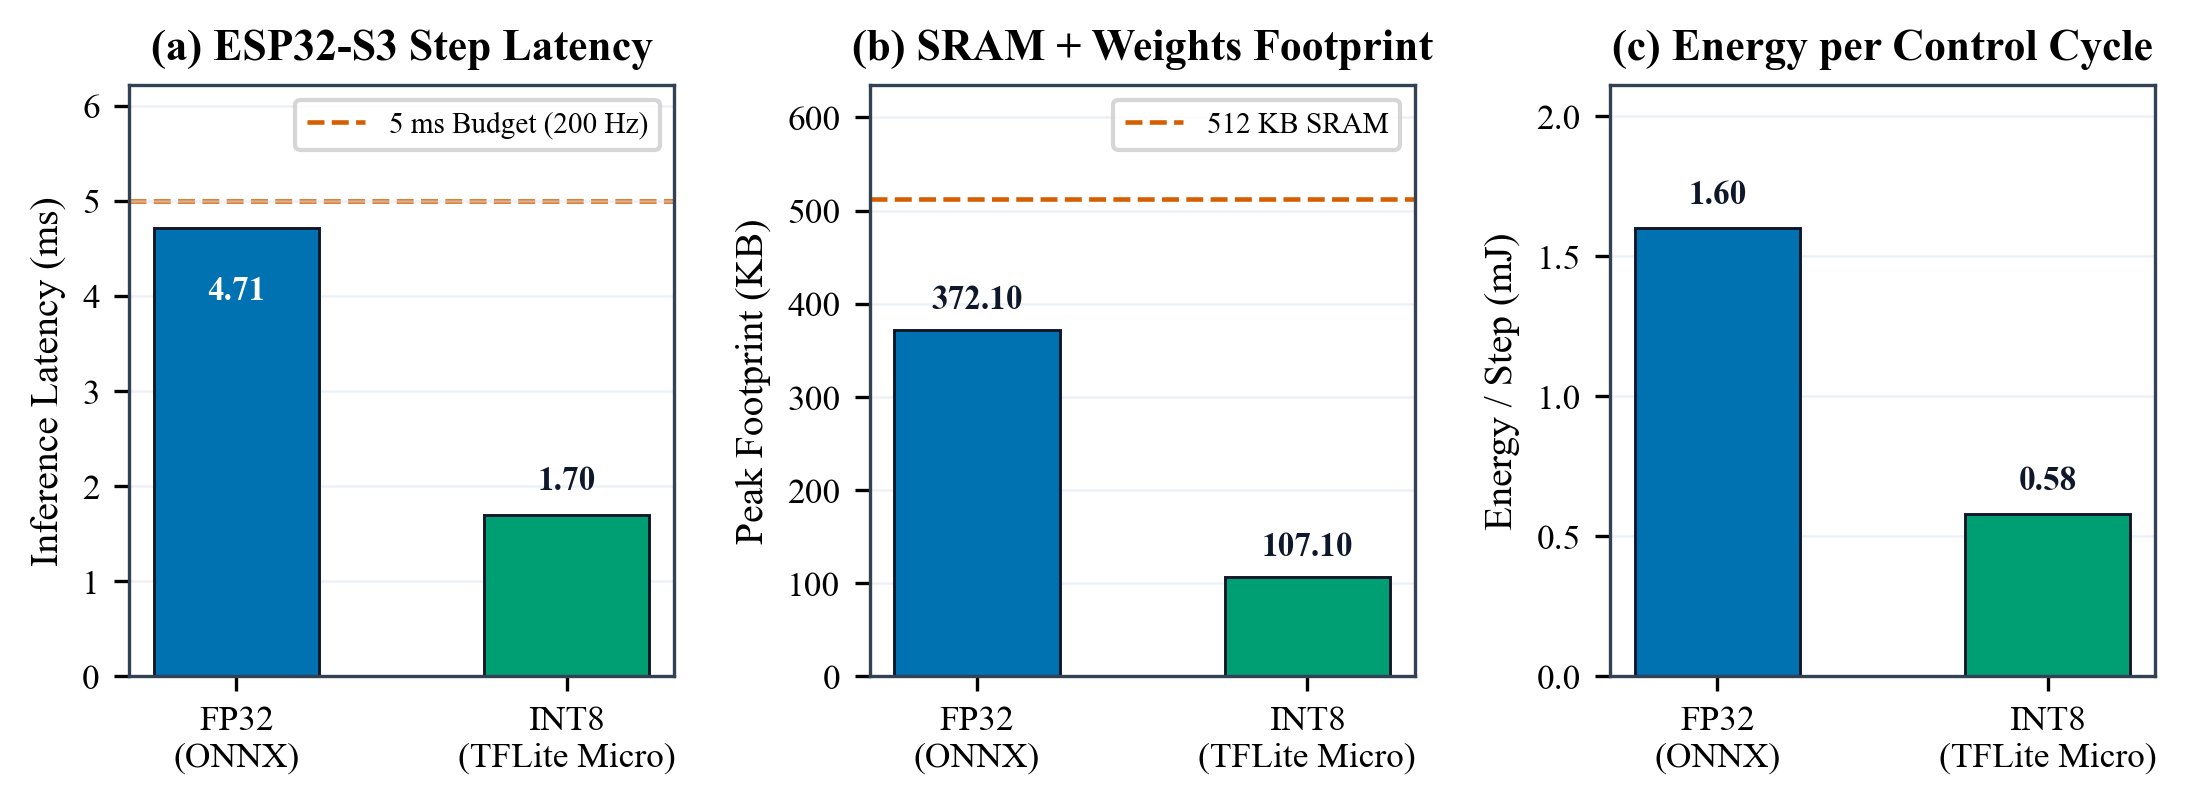
\includegraphics[width=\columnwidth]{../results/figures/fig4_esp32_edge_profiling.png}
    \caption{ESP32-S3 edge inference latency, memory footprint, and energy consumption comparing FP32 ONNX against INT8 TFLite Micro deployment.}
    \label{fig:edge}
\end{figure}

\section{Limitations & Future Work}
First, our outer decision loop steps at 10~Hz matching native USDOT NGSIM camera sampling, which leaves a 4.0\% residual collision rate under dense aggressive cut-ins on unseen I-80 when adjacent lateral encroachment exceeds single-step nudging margins. Second, the ESP32-S3 latency and energy metrics are analytical cycle-count projections validated alongside host CPU ONNX/PyTorch benchmarks rather than physical hardware-in-the-loop (HIL) current probe captures. Future work will incorporate direct 200~Hz C++ closed-loop HIL benchmarking on physical ESP32-S3 boards and cooperative multi-CAV consensus filtering.

\begin{thebibliography}{9}
\bibitem{ngsim}
U.S. Department of Transportation, Federal Highway Administration, ``Next Generation Simulation (NGSIM) Vehicle Trajectories and Supporting Data,'' DOI: \url{10.21949/1504477}.
\bibitem{spmd}
U.S. Department of Transportation, ``Safety Pilot Model Deployment Data,'' DOI: \url{10.21949/1504482}.
\bibitem{ames_cbf}
A.~D. Ames \textit{et al.}, ``Control barrier functions: Theory and applications,'' in \textit{Proc. European Control Conf. (ECC)}, 2019, pp. 3420--3431.
\bibitem{schulman_ppo}
J.~Schulman \textit{et al.}, ``Proximal policy optimization algorithms,'' \textit{arXiv:1707.06347}, 2017.
\end{thebibliography}

\end{document}
